\section{ANALISIS E INTERPRETACION DE RESULTADOS} 

\par A lo largo del desarrollo de este laboratorio, se realizaron difenrentes consultas con PIVOT y Grouping Sets .\\
El resultado de las consultas mencionadas se mostraran a continuacion:


\begin{enumerate}[1.]
	\item Escribiendo consultas con el operador PIVOT
	\begin{enumerate}[a)]
	\item Paso 1: Escribir una sentencia SELECT para recuperar el numero de clientes para un grupo especifico de clientes.\\
		-  Comparamos el resultado de la primera consulta con la que se modifico aplicando el operador PIVOT.
		\begin{figure}[H]
		\begin{center}
		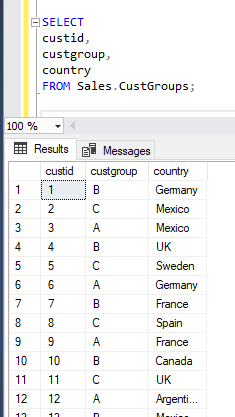
\includegraphics[width=4cm]{./Imagenes/1-2}
		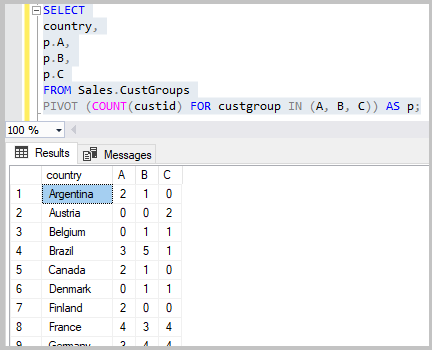
\includegraphics[width=6cm]{./Imagenes/1-3}
		\end{center}
		\end{figure}

	\item Paso 2: Especifique el elemento de agrupacion para el operador PIVOT. \\
		-  Ejecutamos la siguiente consulta, y vemos que su resultado se parece al del paso 1, sin embargo no es lo mismo. Màs filas se devolvieron despues de modificar la vista.
		\begin{figure}[H]
		\begin{center}
		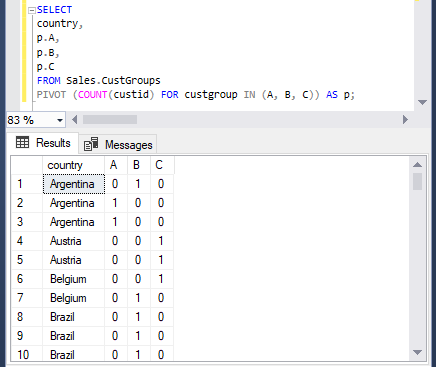
\includegraphics[width=7cm]{./Imagenes/e1-2-1}
		\end{center}
		\end{figure}
		-  Modificar la consulta para incluir columnas adicionales desde la vista y ejecutar; notamos que es el mismo resultado que la consulta anterior. El operador PIVOT asume que todas las columnas excepto la de agregacion y elementos de extension son parte de la agrupacion de columnas.
		\begin{figure}[H]
		\begin{center}
		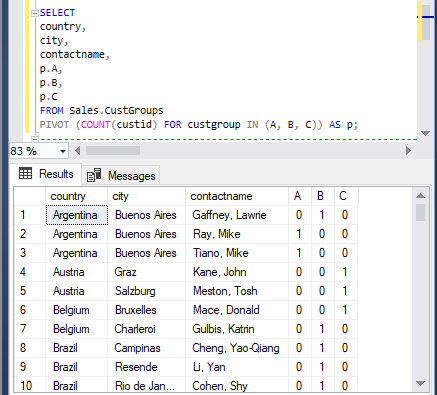
\includegraphics[width=7cm]{./Imagenes/e1-2-2}
		\end{center}
		\end{figure}
	\item Paso 3: Use una expresion de tabla común (CTE) para especificar el elemento de agrupacion para el operador PIVOT.\\
		-  Escribir la siguiente consulta y ejecutar. Se puede observar que el resultado es el mismo que el del paso1; en este paso, la CTE da 3 posibles columnas al operador PIVOT. Y en el paso1, la vista tambien provee 3 columnas a operador PIVOT.
		\begin{figure}[H]
		\begin{center}
		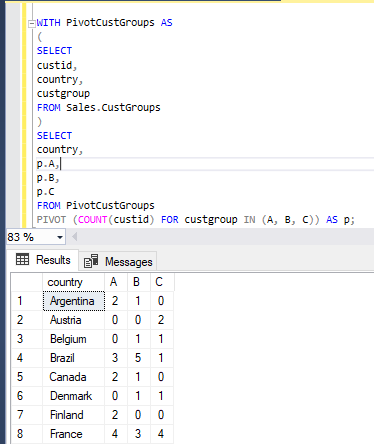
\includegraphics[width=7cm]{./Imagenes/3-1}
		\end{center}
		\end{figure}
		Cuando usamos el operador PIVOT, no puede especificar directamente el elemento de agrupación porque SQL Server asume automáticamente que todas las columnas deben usarse como elementos de agrupación, con la excepción de los elementos de expansión y agregación. Con un CTE, puede especificar las columnas exactas y, por lo tanto, controlar el uso de las columnas para la agrupación.\\
	\item Paso 4: Escribe una instruccion SELECT para recuperar el monto total de ventas para cada cliente y categoria de producto.\\
		-  Escribir la siguiente consulta y ejecutar. 
		\begin{figure}[H]
		\begin{center}
		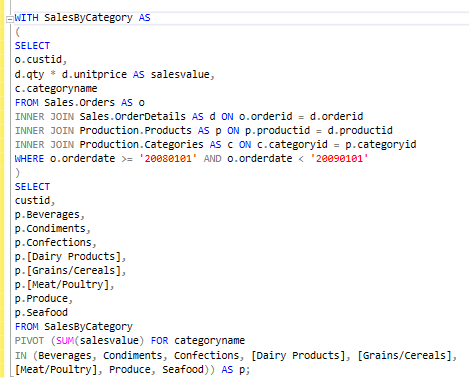
\includegraphics[width=8cm]{./Imagenes/3-2}\\
		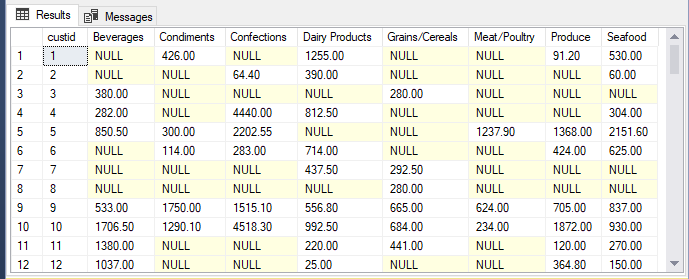
\includegraphics[width=8cm]{./Imagenes/3-3}
		\end{center}
		\end{figure}
	\end{enumerate}

	\item Escribiendo consultas con el operador UNPIVOT
	\begin{enumerate}[a)]
	\item Paso 1: Crear y consultar la vista Sale.PivotCustGroups.\\
		
		-  Ejecutar la siguiente consulta.
		\begin{figure}[H]
		\begin{center}
		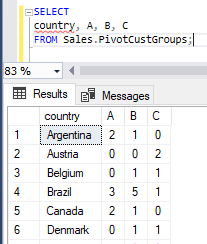
\includegraphics[width=6cm]{./Imagenes/e1-1-1}
		\end{center}
		\end{figure}
	\item Paso 2: Escriba una instruccion SELECT para recuperar una fila para cada pais y grupo de cliente.\\
		-  Escribir la siguiente consulta y ejecutar.\\
		\begin{figure}[H]
		\begin{center}
		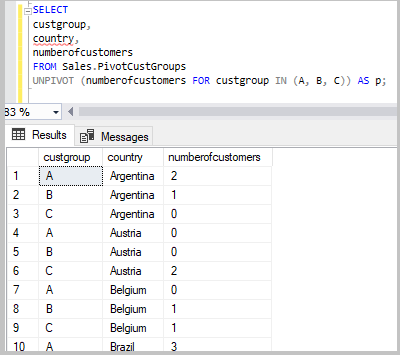
\includegraphics[width=8cm]{./Imagenes/e2-2}
		\end{center}
		\end{figure}
	\end{enumerate}



	\item Escribiendo consultas con las clausulas GROUPING SETS, CUBE, and ROLLUP.
	\begin{enumerate}[a)]
	\item Paso 1: Escriba una instruccion SELECT que use LA SUBCLAUSULA GROUPING SETS para devolver el número de
Clientes para diferentes conjuntos de agrupación.\\
		-  Escribir la siguiente consulta y ejecutar. 
		\begin{figure}[H]
		\begin{center}
		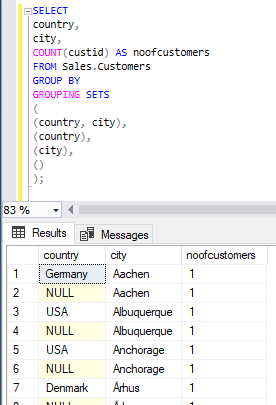
\includegraphics[width=7cm]{./Imagenes/e3-1}
		\end{center}
		\end{figure}
	\item Paso 2: Escriba una instruccion SELECT que use la subclausula CUBE para recuperar Grouping sets basados en valores de ventas anuales, mensuales y diarios.\\
		-  Escribir la siguiente consulta y ejecutar. 
		\begin{figure}[H]
		\begin{center}
		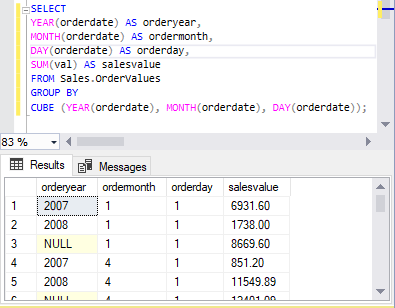
\includegraphics[width=7cm]{./Imagenes/e3-2}
		\end{center}
		\end{figure}
	\item Paso 3: Escriba la misma instruccion SELECT usando la cubclausula ROLLUP.\\
		-  Ejecutalos la siguiente consulta, observamos el resultado. ¿Cuál es la diferencia entre las subcláusulas ROLLUP y CUBE de la cláusula GROUP BY? Al igual que la subcláusula CUBE, la subcláusula ROLLUP proporciona una forma abreviada de definir conjuntos de agrupación múltiples. Sin embargo, a diferencia de CUBE, ROLLUP no produce todos los conjuntos de agrupación posibles que pueden definirse en función de los miembros de entrada, sino que produce un subconjunto de ellos. ROLLUP asume una jerarquía entre los miembros de entrada y produce todos los conjuntos de agrupación que tienen sentido, teniendo en cuenta la jerarquía. En otras palabras, mientras CUBE (a, b, c) produce los ocho conjuntos de agrupación posibles de los tres miembros de entrada, ROLLUP (a, b, c) produce solo cuatro conjuntos de agrupación, asumiendo la jerarquía a> b> c. ROLLUP (a, b, c) es el equivalente a especificar CONJUNTOS DE AGRUPACIÓN ((a, b, c), (a, b), (a), ()).
¿Cuál es la subcláusula más apropiada para usar en este ejemplo? Desde año, mes y día forman un
Jerarquía, la cláusula ROLLUP es más adecuada. Probablemente no hay mucho interés en mostrar
se acumula durante un mes independientemente del año, pero al revés es interesante.
		\begin{figure}[H]
		\begin{center}
		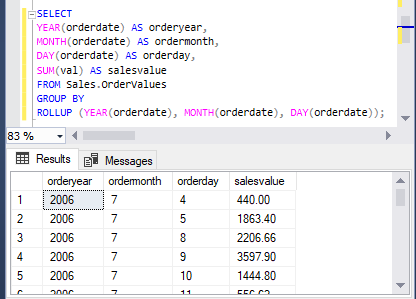
\includegraphics[width=7cm]{./Imagenes/e3-3}
		\end{center}
		\end{figure}
	\item Paso 4: Analizar el valor total de ventas por año y mes.\\
		-  Escribir la siguiente consulta y ejecutar. 
		\begin{figure}[H]
		\begin{center}
		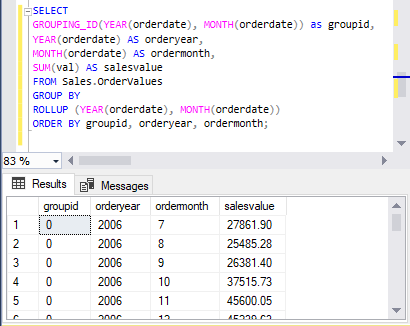
\includegraphics[width=7cm]{./Imagenes/e3-4}
		\end{center}
		\end{figure}
	\end{enumerate}
\end{enumerate}

